%% Beispiel-Präsentation mit LaTeX Beamer im KIT-Design
%% entsprechend den Gestaltungsrichtlinien vom 1. August 2020
%%
%% Siehe https://sdqweb.ipd.kit.edu/wiki/Dokumentvorlagen

%% Beispiel-Präsentation
\documentclass[en]{sdqbeamer}

\usepackage{xcolor}
\definecolor{backcolour}{rgb}{0.95,0.95,0.92}
\definecolor{codegray}{rgb}{0.5,0.5,0.5}

\usepackage{multicol}
\usepackage{subcaption}

\usepackage{listings}
\lstdefinestyle{mystyle}{
    backgroundcolor=\color{backcolour},
    basicstyle=\ttfamily\footnotesize,
    breakatwhitespace=false,
    breaklines=true,
    keepspaces=true,
    numbers=left,
    numbersep=5pt,
    numberstyle=\tiny\color{codegray},
    showspaces=false,
    showstringspaces=false,
    showtabs=false,
    tabsize=2
}
\lstset{style=mystyle}

\usepackage{graphicx}
\graphicspath{ {./figures/} }

\titleimage{banner_2020_kit}

\grouplogo{}

\groupname{EML-lab}
%\groupnamewidth{50mm}


\title[EML-lab]{Embedded Machine Learning Lab}
\author[Max Schik, Darius Schefer]{Max Schik, Darius Schefer}

\date[03/20/2024]{March 20, 2024}

\begin{document}

\KITtitleframe

\begin{frame}{Contents}
  \tableofcontents
\end{frame}

\begin{frame}{Cat}
  \begin{figure}
    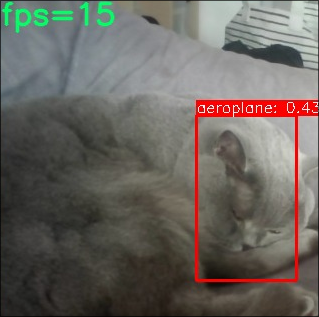
\includegraphics[scale=0.55]{kira_detection}
  \end{figure}
\end{frame}

\section{Data}
\begin{frame}[t]{Data}
  \begin{columns}
    \begin{column}{0.45\textwidth}
      \begin{itemize}
      \item More data
        \begin{itemize}
        \item Human Dataset
          \footnote{https://www.kaggle.com/datasets/fareselmenshawii/human-dataset} (17,300 images)
        \item Tiktok Dancing
          \footnote{https://www.kaggle.com/datasets/tapakah68/segmentation-full-body-tiktok-dancing-dataset} (2615 images)
        \end{itemize}

      \item Data augmentation
        \begin{itemize}
        \item Albumentations\footnote{https://albumentations.ai/} library
        \item Rotation, flipping, contrast
        \end{itemize}
      \end{itemize}
    \end{column}
    \begin{column}{0.55\textwidth}
      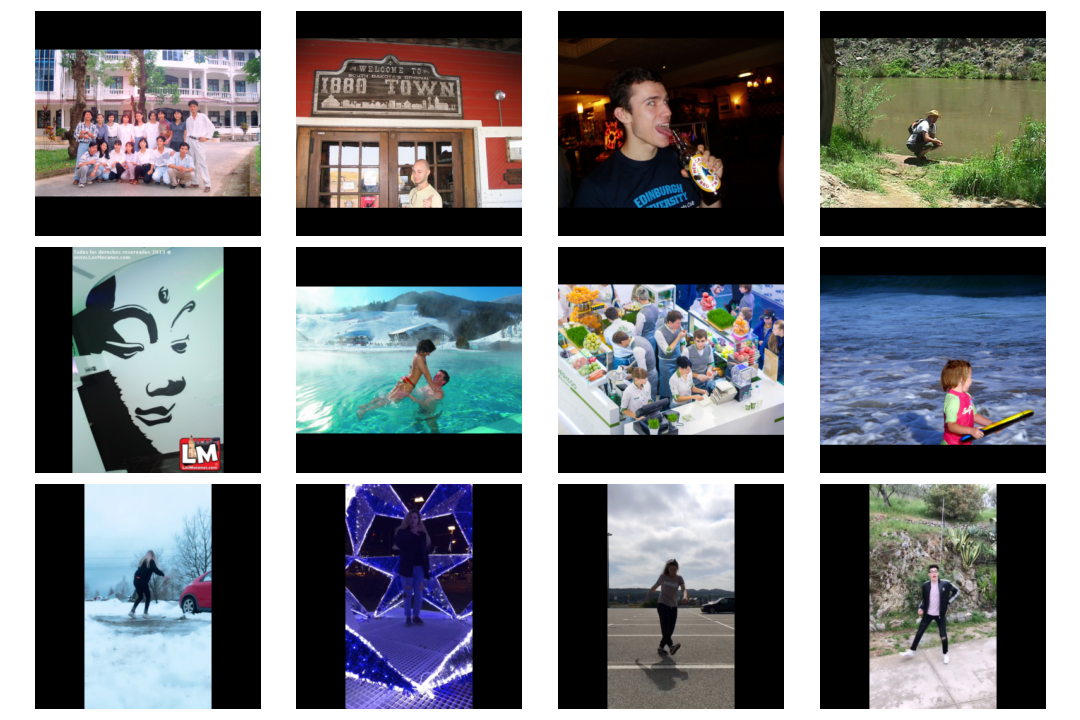
\includegraphics[scale=0.22]{data_grid}
    \end{column}
  \end{columns}
\end{frame}

\section{Adaptation and optimization}
\begin{frame}{Adaptation and optimization}
  \begin{columns}
    \begin{column}{0.4\textwidth}
      \begin{itemize}
        \item Person-only-detection, fine-tuning
        \item Iterative pruning
        \item Batch norm optimization
        \item Inference
      \end{itemize}
    \end{column}
    \begin{column}{0.6\textwidth}
      \begin{figure}
        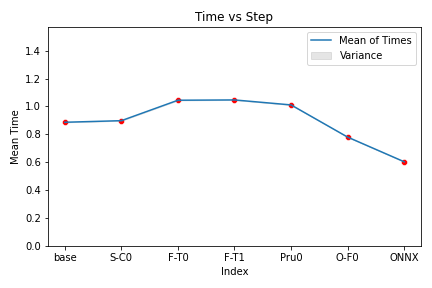
\includegraphics[scale=0.5]{time_against_step}
      \end{figure}
    \end{column}
  \end{columns}
\end{frame}

\begin{frame}{Inference}
  \begin{columns}
    \begin{column}{0.4\textwidth}
      \begin{itemize}
        \item ONNX
        \item TensorRT
        \begin{itemize}
          \item TensorRT supports only a subset of ONNX spec
          \item \texttt{ReflectivePad} $\rightarrow{}$ \texttt{ConstantPad}
          \item Simplification of graph with \texttt{onnx-simplifier}\footnote{\url{https://github.com/daquexian/onnx-simplifier}}
        \end{itemize}
      \end{itemize}
    \end{column}
    \begin{column}{0.6\textwidth}
      \begin{figure}
        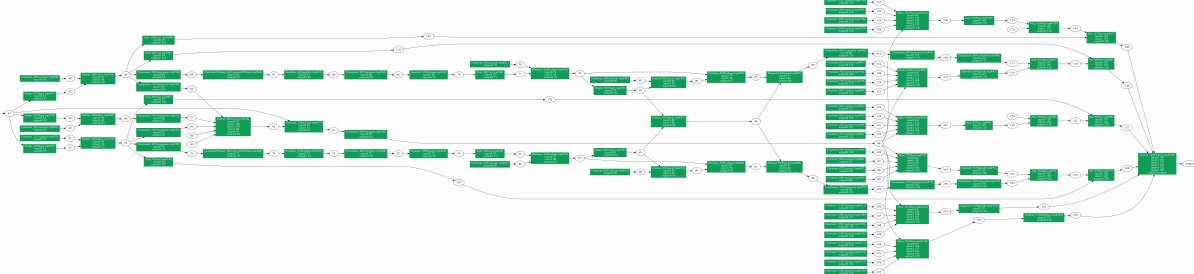
\includegraphics[width=\columnwidth]{complex_graph.png}
        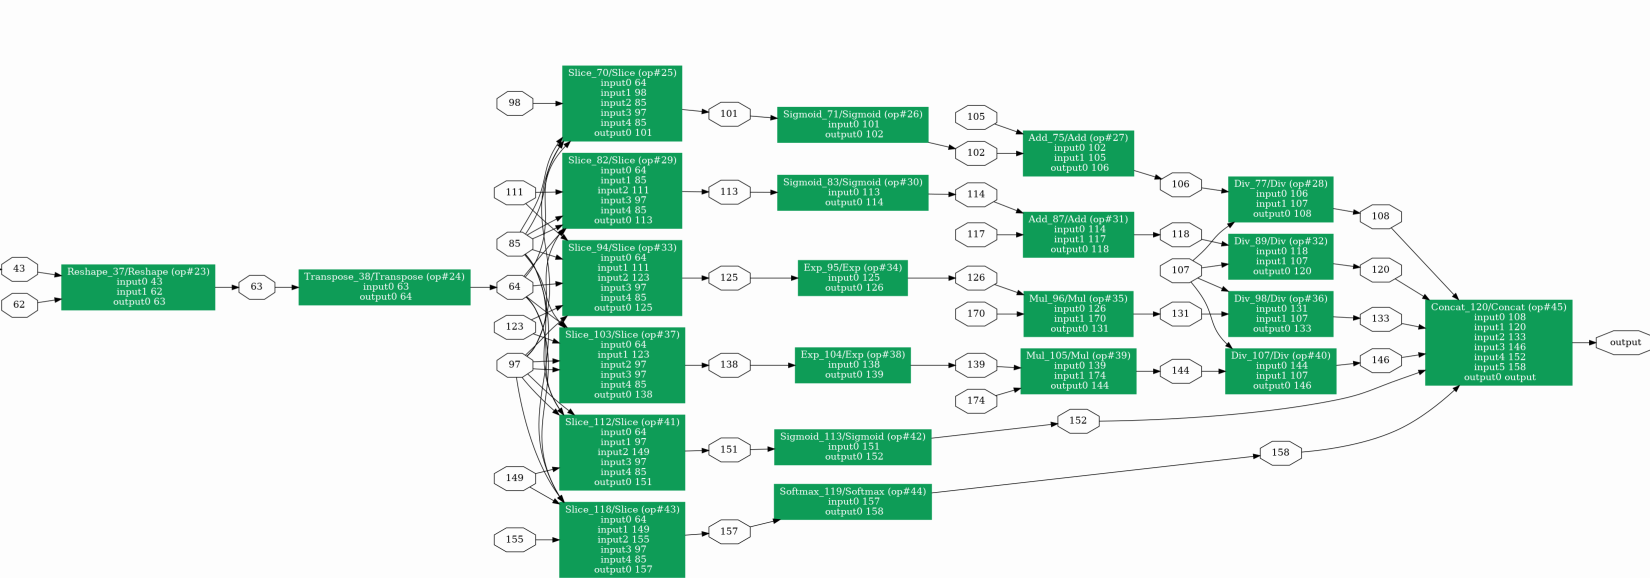
\includegraphics[width=\columnwidth]{simplified_graph.png}
      \end{figure}
    \end{column}
  \end{columns}
\end{frame}

\begin{frame}%[plain]
  \begin{figure}
    \centering
    \begin{subfigure}{0.45\textwidth}
      \centering
      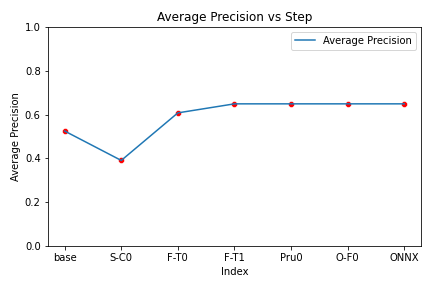
\includegraphics[scale=0.35]{average_precision_against_step}
    \end{subfigure}
    \hfill
    \begin{subfigure}{0.45\textwidth}
      \centering
      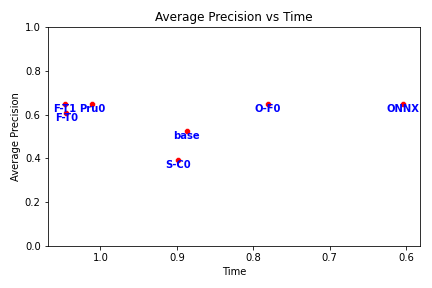
\includegraphics[scale=0.35]{average_precision_against_time}
    \end{subfigure}
    \vskip\baselineskip
    \begin{subfigure}{0.45\textwidth}
      \centering
      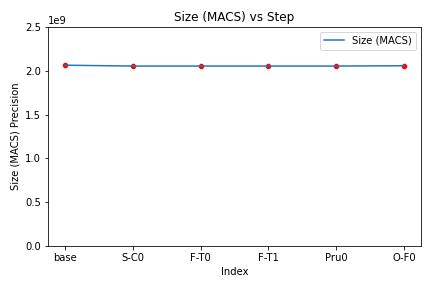
\includegraphics[scale=0.35]{size_against_step}
    \end{subfigure}
    \hfill
    \begin{subfigure}{0.45\textwidth}
      \centering
      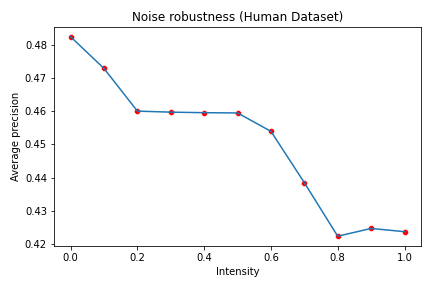
\includegraphics[scale=0.35]{noise_robustness}
    \end{subfigure}
  \end{figure}
\end{frame}

\begin{frame}{Detections}
  \begin{figure}
    \centering
    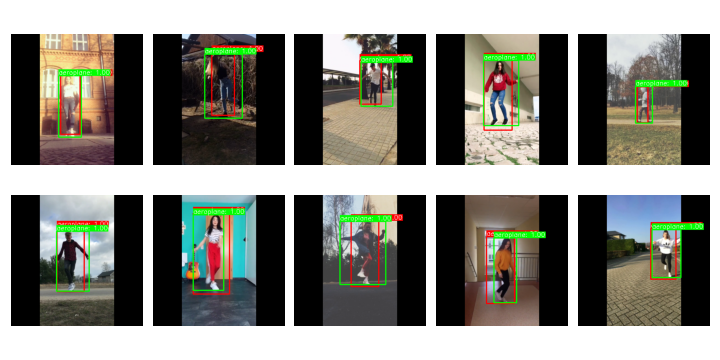
\includegraphics[scale=0.5]{detections}
  \end{figure}
\end{frame}

\section{Integration and pipeline}
\begin{frame}[fragile]{Integration and pipeline}
  \begin{columns}
    \begin{column}{0.5\textwidth}
      \begin{itemize}
      \item Configuration
        \begin{itemize}
        \item File containing steps and parameters
        \item Reproducibility
        \item Version control
        \end{itemize}
      \item Camera loop
        \begin{itemize}
        \item TensorRT for faster inference
        \item Avg. 20fps
        \end{itemize}
      \end{itemize}
    \end{column}

    \begin{column}{0.5\textwidth}
      \begin{lstlisting}
--- !experiment
start_weights_path: "./weights/voc_pretrained.pt"
augment: True

steps:
- !strip_classes
    finetune: true
    finetune_epochs: 15
- !pruning
    target_acc: 0.3
    prune_ratio: 0.05
    batch_size: 64
    num_train_epochs: 10
    num_eval_batches: 10
- !operator_fusion {}
      \end{lstlisting}
    \end{column}
  \end{columns}
\end{frame}

\section{Live demo}
\begin{frame}
  \begin{center}
    \huge{Live Demo}
  \end{center}
\end{frame}

\end{document}
